%%
%% This is file `mcmthesis-demo.tex',
%% generated with the docstrip utility.
%%
%% The original source files were:
%%
%% mcmthesis.dtx  (with options: `demo')
%%
%% -----------------------------------
%%
%% This is a generated file.
%%
%% Copyright (C)
%%       2010 -- 2015 by Zhaoli Wang
%%       2014 -- 2019 by Liam Huang
%%       2019 -- present by latexstudio.net
%%
%% This work may be distributed and/or modified under the
%% conditions of the LaTeX Project Public License, either version 1.3
%% of this license or (at your option) any later version.
%% The latest version of this license is in
%%   http://www.latex-project.org/lppl.txt
%% and version 1.3 or later is part of all distributions of LaTeX
%% version 2005/12/01 or later.
%%
%% This work has the LPPL maintenance status `maintained'.
%%
%% The Current Maintainer of this work is Liam Huang.
%%
%%
%% This is file `mcmthesis-demo.tex',
%% generated with the docstrip utility.
%%
%% The original source files were:
%%
%% mcmthesis.dtx  (with options: `demo')
%%
%% -----------------------------------
%%
%% This is a generated file.
%%
%% Copyright (C)
%%       2010 -- 2015 by Zhaoli Wang
%%       2014 -- 2019 by Liam Huang
%%       2019 -- present by latexstudio.net
%%
%% This work may be distributed and/or modified under the
%% conditions of the LaTeX Project Public License, either version 1.3
%% of this license or (at your option) any later version.
%% The latest version of this license is in
%%   http://www.latex-project.org/lppl.txt
%% and version 1.3 or later is part of all distributions of LaTeX
%% version 2005/12/01 or later.
%%
%% This work has the LPPL maintenance status `maintained'.
%%
%% The Current Maintainer of this work is Liam Huang.
%%
\documentclass{mcmthesis}
\mcmsetup{CTeX = false,    % 使用 CTeX 套装时,设置为 true
          tcn = {0000000}, problem = \textcolor{red}{A},
          sheet = true, titleinsheet = true, keywordsinsheet = true,
          titlepage = false, abstract = false}
        
\usepackage{newtxtext}     % \usepackage{palatino}
\usepackage[backend=bibtex]{biblatex}   % for RStudio Complie

\usepackage{tocloft}
\setlength{\cftbeforesecskip}{6pt}
\renewcommand{\contentsname}{\hspace*{\fill}\Large\bfseries Contents \hspace*{\fill}}

\title{Enjoy a Cozy and Green Bath}
% \author{\small \href{http://www.latexstudio.net/}
%   {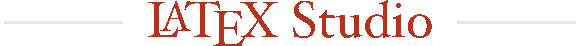
\includegraphics[width=7cm]{mcmthesis-logo}}}
\date{\today}

\begin{document}

\begin{abstract}

A traditional bathtub cannot be reheated by itself, so users have to add hot water from time to time. Our goal is to establish a model of the temperature of bath water in space and time. Then we are expected to propose an optimal strategy for users to keep the temperature even and close to initial temperature and decrease water consumption.

To simplify modeling process, we firstly assume there is no person in the bathtub. We regard the whole bathtub as a thermodynamic system and introduce heat transfer formulas.

We establish two sub-models: adding water constantly and discontinuously. As for the former sub-model, we define the mean temperature of bath water. Introducing Newton cooling formula, we determine the heat transfer capacity. After deriving the value of parameters, we deduce formulas to derive results and simulate the change of temperature field via CFD. As for the second sub-model, we define an iteration consisting of two process: heating and standby. According to energy conservation law, we obtain the relationship of time and total heat dissipating capacity. Then we determine the mass flow and the time of adding hot water. We also use CFD to simulate the temperature field in second sub-model.

In consideration of evaporation, we correct the results of sub-models referring to some scientists' studies. We define two evaluation criteria and compare the two sub-models. Adding water constantly is found to keep the temperature of bath water even and avoid wasting too much water, so it is recommended by us.

Then we determine the influence of some factors: radiation heat transfer, the shape and volume of the tub, the shape/volume/temperature/motions of the person, the bubbles made from bubble bath additives. We focus on the influence of those factors to heat transfer and then conduct sensitivity analysis. The results indicate smaller bathtub with less surface area, lighter personal mass, less motions and more bubbles will decrease heat transfer and save water.

Based on our model analysis and conclusions, we propose the optimal strategy for the user in a bathtub and explain the reason of uneven temperature throughout the bathtub. In addition, we make improvement for applying our model in real life.

\begin{keywords}
Heat transfer, Thermodynamic system, CFD, Energy conservation
\end{keywords}

\end{abstract}

\maketitle

%% Generate the Table of Contents, if it's needed.
% \renewcommand{\contentsname}{\centering Contents}
\tableofcontents   % 若不想要目录, 注释掉该句
\thispagestyle{empty}

\newpage


\section{Introduction}

\subsection{Background}

Bathing in a tub is a perfect choice for those who have been worn out after a long day's working. A traditional bathtub is a simply water containment vessel without a secondary heating system or circulating jets. Thus the temperature of water in bathtub declines noticeably as time goes by, which will influent the experience of bathing. As a result, the bathing person needs to add a constant trickle of hot water from a faucet to reheat the bathing water. This way of bathing will result in waste of water because when the capacity of the bathtub is reached, excess water overflows the tub.

An optimal bathing strategy is required for the person in a bathtub to get comfortable bathing experience while reducing the waste of water.

\subsection{Literature Review}

Korean physicist Gi-Beum Kim analyzed heat loss through free surface of water contained in bathtub due to conduction and evaporation \cite{1}. He derived a relational equation based on the basic theory of heat transfer to evaluate the performance of bath tubes. The major heat loss was found to be due to evaporation. Moreover, he found out that the speed of heat loss depends more on the humidity of the bathroom than the temperature of water contained in the bathtub. So, it is best to maintain the temperature of bathtub water to be between 41 to 45$^{\circ}$C and the humidity of bathroom to be 95\%.

When it comes to convective heat transfer in bathtub, many studies can be referred to. Newton's law of cooling states that the rate of heat loss of a body is proportional to the difference in temperatures between the body and its surroundings while under the effects of a breeze \cite{2}. Claude-Louis Navier and George Gabriel Stokes described the motion of viscous fluid substances with the Navier-Stokes equations. Those equations may be used to model the weather, ocean currents, water flow in a pipe and air flow around a wing \cite{3}.

In addition, some numerical simulation software are applied in solving and analyzing problems that involve fluid flows. For example, Computational Fluid Dynamics (CFD) is a common one used to perform the calculations required to simulate the interaction of liquids and gases with surfaces defined by boundary conditions \cite{4}.

\subsection{Restatement of the Problem}

We are required to establish a model to determine the change of water temperature in space and time. Then we are expected to propose the best strategy for the person in the bathtub to keep the water temperature close to initial temperature and even throughout the tub. Reduction of waste of water is also needed. In addition, we have to consider the impact of different conditions on our model, such as different shapes and volumes of the bathtub, etc.

In order to solve those problems, we will proceed as follows:

\begin{itemize}
\item {\bf Stating assumptions}. By stating our assumptions, we will narrow the focus of our approach towards the problems and provide some insight into bathtub water temperature issues.

\item {\bf Making notations}. We will give some notations which are important for us to clarify our models.

\item {\bf Presenting our model}. In order to investigate the problem deeper, we divide our model into two sub-models. One is a steady convection heat transfer sub-model in which hot water is added constantly. The other one is an unsteady convection heat transfer sub-model where hot water is added discontinuously.

\item {Defining evaluation criteria and comparing sub-models}. We define two main criteria to evaluate our model: the mean temperature of bath water and the amount of inflow water.

\item {\bf Analysis of influencing factors}. In term of the impact of different factors on our model, we take those into consideration: the shape and volume of the tub, the shape/volume/temperature of the person in the bathtub, the motions made by the person in the bathtub and adding a bubble bath additive initially.

\item {\bf Model testing and sensitivity analysis}. With the criteria defined before, we evaluate the reliability of our model and do the sensitivity analysis.

\item {\bf Further discussion}. We discuss about different ways to arrange inflow faucets. Then we improve our model to apply them in reality.

\item {\bf Evaluating the model}. We discuss about the strengths and weaknesses of our model:

\begin{itemize}
\item[1)] ... 
\item[2)] ...
\item[3)] ...
\item[4)] ...
\end{itemize}

\end{itemize}

\section{Assumptions and Justification}

To simplify the problem and make it convenient for us to simulate real-life conditions, we make the following basic assumptions, each of which is properly justified.

\begin{itemize}
\item {\bf The bath water is incompressible Non-Newtonian fluid}. The incompressible Non-Newtonian fluid is the basis of Navier–Stokes equations which are introduced to simulate the flow of bath water.

\item {\bf All the physical properties of bath water, bathtub and air are assumed to be stable}. The change of those properties like specific heat, thermal conductivity and density is rather small according to some studies \cite{5}. It is complicated and unnecessary to consider these little change so we ignore them.

\item {\bf There is no internal heat source in the system consisting of bathtub, hot water and air}. Before the person lies in the bathtub, no internal heat source exist except the system components. The circumstance where the person is in the bathtub will be investigated in our later discussion.

\item {\bf We ignore radiative thermal exchange}. According to Stefan-Boltzmann’s law, the radiative thermal exchange can be ignored when the temperature is low. Refer to industrial standard \cite{6}, the temperature in bathroom is lower than 100 $^{\circ}$C, so it is reasonable for us to make this assumption.

\item {\bf The temperature of the adding hot water from the faucet is stable}. This hypothesis can be easily achieved in reality and will simplify our process of solving the problem.
\end{itemize}

\section{Notations}

\begin{center}
\begin{tabular}{clc}
{\bf Symbols} & {\bf Description} & \quad {\bf Unit} \\[0.25cm]
$h$ & Convection heat transfer coefficient & \quad W/(m$^2 \cdot$ K) 
\\[0.2cm]
$k$ & Thermal conductivity & \quad W/(m $\cdot$ K) \\[0.2cm]
$c_p$ & Specific heat & \quad J/(kg $\cdot$ K) \\[0.2cm]
$\rho$ & Density & \quad kg/m$^2$ \\[0.2cm]
$\delta$ & Thickness & \quad m \\[0.2cm]
$t$ & Temperature & \quad $^\circ$C, K \\[0.2cm]
$\tau$ & Time & \quad s, min, h \\[0.2cm]
$q_m$ & Mass flow & \quad kg/s \\[0.2cm]
$\Phi$ & Heat transfer power & \quad W \\[0.2cm]
$T$ & A period of time & \quad s, min, h \\[0.2cm]
$V$ & Volume & \quad m$^3$, L \\[0.2cm]
$M,\,m$ & Mass & \quad kg \\[0.2cm]
$A$ & Aera & \quad m$^2$ \\[0.2cm]
$a,\,b,\,c$ & The size of a bathtub  & \quad m$^3$
\end{tabular}
\end{center}

\noindent where we define the main parameters while specific value of those parameters will be given later.

\section{Model Overview}

In our basic model, we aim at three goals: keeping the temperature as even as possible, making it close to the initial temperature and decreasing the water consumption.

We start with the simple sub-model where hot water is added constantly.
At first we introduce convection heat transfer control equations in rectangular coordinate system. Then we define the mean temperature of bath water.

Afterwards, we introduce Newton cooling formula to determine heat transfer
capacity. After deriving the value of parameters, we get calculating results via formula deduction and simulating results via CFD.

Secondly, we present the complicated sub-model in which hot water is
added discontinuously. We define an iteration consisting of two process:
heating and standby. As for heating process, we derive control equations and boundary conditions. As for standby process, considering energy conservation law, we deduce the relationship of total heat dissipating capacity and time.

Then we determine the time and amount of added hot water. After deriving the value of parameters, we get calculating results via formula deduction and simulating results via CFD.

At last, we define two criteria to evaluate those two ways of adding hot water. Then we propose optimal strategy for the user in a bathtub.
The whole modeling process can be shown as follows.

\begin{figure}[h] 
\centering
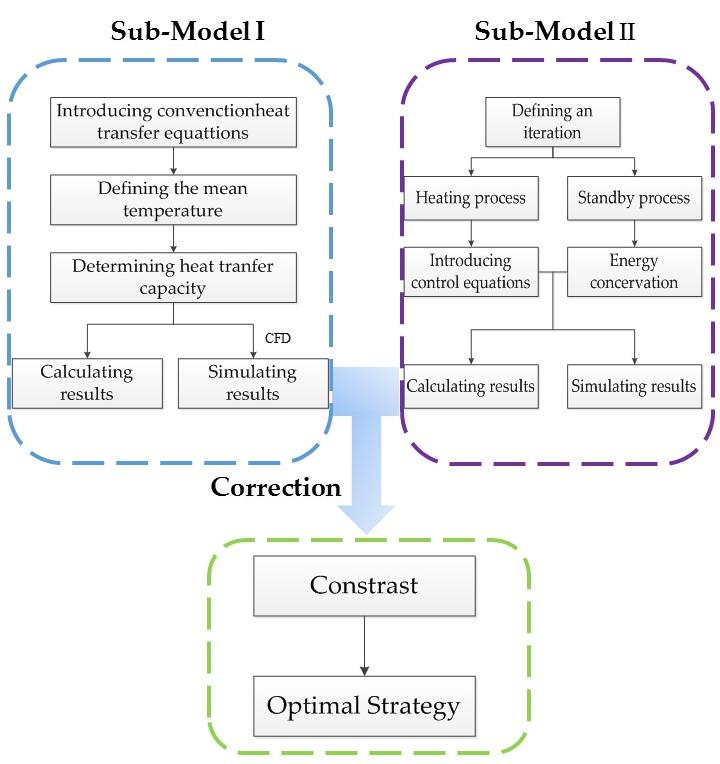
\includegraphics[width=12cm]{fig1.jpg}
\caption{Modeling process} \label{fig1}
\end{figure}

\section{Sub-model I : Adding Water Continuously}

We first establish the sub-model based on the condition that a person add water continuously to reheat the bathing water. Then we use Computational Fluid Dynamics (CFD) to simulate the change of water temperature in the bathtub. At last, we evaluate the model with the criteria which have been defined before.

\subsection{Model Establishment}

Since we try to keep the temperature of the hot water in bathtub to be even, we have to derive the amount of inflow water and the energy dissipated by the hot water into the air.

We derive the basic convection heat transfer control equations based on the former scientists’ achievement. Then, we define the mean temperature of bath water. Afterwards, we determine two types of heat transfer: the boundary heat transfer and the evaporation heat transfer. Combining thermodynamic formulas, we derive calculating results. Via Fluent software, we get simulation results.

\subsubsection{Control Equations and Boundary Conditions}

According to thermodynamics knowledge, we recall on basic convection
heat transfer control equations in rectangular coordinate system. Those
equations show the relationship of the temperature of the bathtub water in space.

We assume the hot water in the bathtub as a cube. Then we put it into a
rectangular coordinate system. The length, width, and height of it is $a,\, b$ and $c$.

\begin{figure}[h] 
\centering
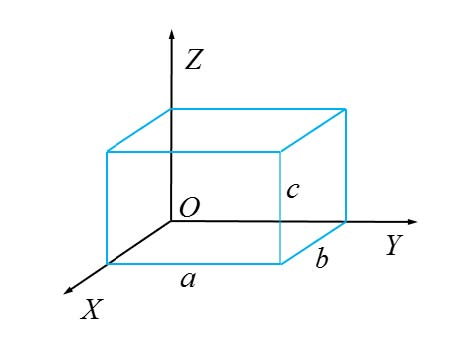
\includegraphics[width=8cm]{fig2.jpg}
\caption{Modeling process} \label{fig2}
\end{figure}

In the basis of this, we introduce the following equations \cite{5}:

\begin{itemize}
\item {\bf Continuity equation:}
\end{itemize}

\begin{equation} \label{eq1}
\frac{\partial u}{\partial x} + \frac{\partial v}{\partial y} +\frac{\partial w}{\partial z} =0
\end{equation}

\noindent where the first component is the change of fluid mass along the $X$-ray. The second component is the change of fluid mass along the $Y$-ray. And the third component is the change of fluid mass along the $Z$-ray. The sum of the change in mass along those three directions is zero.

\begin{itemize}
\item {\bf Moment differential equation (N-S equations):}
\end{itemize}

\begin{equation} \label{eq2}
\left\{
\begin{array}{l} \!\!
\rho \Big(u \dfrac{\partial u}{\partial x} + v \dfrac{\partial u}{\partial y} + w\dfrac{\partial u}{\partial z} \Big) = -\dfrac{\partial p}{\partial x} + \eta \Big(\dfrac{\partial^2 u}{\partial x^2} + \dfrac{\partial^2 u}{\partial y^2} + \dfrac{\partial^2 u}{\partial z^2} \Big) \\[0.3cm]
\rho \Big(u \dfrac{\partial v}{\partial x} + v \dfrac{\partial v}{\partial y} + w\dfrac{\partial v}{\partial z} \Big) = -\dfrac{\partial p}{\partial y} + \eta \Big(\dfrac{\partial^2 v}{\partial x^2} + \dfrac{\partial^2 v}{\partial y^2} + \dfrac{\partial^2 v}{\partial z^2} \Big) \\[0.3cm]
\rho \Big(u \dfrac{\partial w}{\partial x} + v \dfrac{\partial w}{\partial y} + w\dfrac{\partial w}{\partial z} \Big) = -g-\dfrac{\partial p}{\partial z} + \eta \Big(\dfrac{\partial^2 w}{\partial x^2} + \dfrac{\partial^2 w}{\partial y^2} + \dfrac{\partial^2 w}{\partial z^2} \Big)  
\end{array}
\right.
\end{equation}

\begin{itemize}
\item {\bf Energy differential equation:}
\end{itemize}

\begin{equation} \label{eq3}
\rho c_p \Big( u\frac{\partial t}{\partial x} + v\frac{\partial t}{\partial y} + w\frac{\partial t}{\partial z} \Big) = \lambda \Big(\frac{\partial^2 t}{\partial x^2} + \frac{\partial^2 t}{\partial y^2} + \frac{\partial^2 t}{\partial z^2} \Big)
\end{equation}

\noindent where the left three components are convection terms while the right three components are conduction terms.

By Equation \eqref{eq3}, we have ......

......

On the right surface in Fig. \ref{fig2}, the water also transfers heat firstly with bathtub inner surfaces and then the heat comes into air. The boundary condition here is ......

\subsubsection{Definition of the Mean Temperature}

......

\subsubsection{Determination of Heat Transfer Capacity}

......

\section{Sub-model II: Adding Water Discontinuously}

In order to establish the unsteady sub-model, we recall on the working principle of air conditioners. The heating performance of air conditions consist of two processes: heating and standby. After the user set a temperature, the air conditioner will begin to heat until the expected temperature is reached. Then it will go standby. When the temperature get below the expected temperature, the air conditioner begin to work again. As it works in this circle, the temperature remains the expected one.

Inspired by this, we divide the bathtub working into two processes: adding
hot water until the expected temperature is reached, then keeping this
condition for a while unless the temperature is lower than a specific value. Iterating this circle ceaselessly will ensure the temperature kept relatively stable.

\subsection{Heating Model}

\subsubsection{Control Equations and Boundary Conditions}

\subsubsection{Determination of Inflow Time and Amount}

\subsection{Standby Model}

\subsection{Results}

\quad~ We first give the value of parameters based on others’ studies. Then we get the calculation results and simulating results via those data.

\subsubsection{Determination of Parameters}

After establishing the model, we have to determine the value of some
important parameters.

As scholar Beum Kim points out, the optimal temperature for bath is
between 41 and 45$^\circ$C [1]. Meanwhile, according to Shimodozono's study, 41$^\circ$C warm water bath is the perfect choice for individual health [2]. So it is reasonable for us to focus on $41^\circ$C $\sim 45^\circ$C. Because adding hot water continuously is a steady process, so the mean temperature of bath water is supposed to be constant. We value the temperature of inflow and outflow water with the maximum and minimum temperature respectively.

The values of all parameters needed are shown as follows:

.....

\subsubsection{Calculating Results}

Putting the above value of parameters into the equations we derived before, we can get the some data as follows:

%%普通表格
\begin{table}[h]  %h表示固定在当前位置
\centering        %设置居中
\caption{The calculating results}  %表标题
\vspace{0.15cm}
\label{tab2}                       %设置表的引用标签
\begin{tabular}{|c|c|c|}  %3个c表示3列, |可选, 表示绘制各列间的竖线
\hline                    %画横线
Variables & Values & Unit     \\ \hline  %各列间用&隔开
$A_1$     & 1.05   &   $m^2$  \\ \hline
$A_2$     & 2.24   &   $m^2$  \\ \hline
$\Phi_1$  & 189.00 &   $W$   \\ \hline
$\Phi_2$  & 43.47  &   $W$   \\ \hline
$\Phi$    & 232.47 &   $W$   \\ \hline
$q_m$     & 0.014  &   $g/s$ \\ \hline
\end{tabular}
\end{table}

From Table \ref{tab2}, ......

......

\section{Correction and Contrast of Sub-Models}

After establishing two basic sub-models, we have to correct them in consideration of evaporation heat transfer. Then we define two evaluation criteria to compare the two sub-models in order to determine the optimal bath strategy.

\subsection{Correction with Evaporation Heat Transfer}

Someone may confuse about the above results: why the mass flow in the first sub-model is so small? Why the standby time is so long? Actually, the above two sub-models are based on ideal conditions without consideration of the change of boundary conditions, the motions made by the person in bathtub and the evaporation of bath water, etc. The influence of personal motions will be discussed later. Here we introducing the evaporation of bath water to correct sub-models.

\subsection{Contrast of Two Sub-Models}

Firstly we define two evaluation criteria. Then we contrast the two submodels via these two criteria. Thus we can derive the best strategy for the person in the bathtub to adopt.

\section{Model Analysis and Sensitivity Analysis}

\subsection{The Influence of Different Bathtubs}

Definitely, the difference in shape and volume of the tub affects the
convection heat transfer. Examining the relationship between them can help
people choose optimal bathtubs.

\subsubsection{Different Volumes of Bathtubs}

In reality, a cup of water will be cooled down rapidly. However, it takes quite long time for a bucket of water to become cool. That is because their volume is different and the specific heat of water is very large. So that the decrease of temperature is not obvious if the volume of water is huge. That also explains why it takes 45 min for 320 L water to be cooled by 1$^\circ$C.

In order to examine the influence of volume, we analyze our sub-models
by conducting sensitivity Analysis to them.

We assume the initial volume to be 280 L and change it by $\pm 5$\%, $\pm 8$\%, $\pm 12$\% and $\pm 15$\%. With the aid of sub-models we established before, the variation of some parameters turns out to be as follows

%%三线表
\begin{table}[h] %h表示固定在当前位置
\centering  %设置居中
\caption{Variation of some parameters}  %表标题
\label{tab7} %设置表的引用标签
\begin{tabular}{ccccccc} %7个c表示7列, c表示每列居中对齐, 还有l和r可选
\toprule  %画顶端横线
$V$      & $A_1$   & $A_2$   & $T_2$    & $q_{m1}$ & $q_{m2}$ & $\Phi_q$ \\
\midrule  %画中间横线
-15.00\% & -5.06\% & -9.31\% & -12.67\% & -2.67\%  & -14.14\% & -5.80\% \\
-12.00\% & -4.04\% & -7.43\% & -10.09\% & -2.13\%  & -11.31\% & -4.63\% \\
-8.00\%  & -2.68\% & -4.94\% & -6.68\%  & -1.41\%  & -7.54\%  & -3.07\% \\
-8.00\%  & -2.68\% & -4.94\% & -6.68\%  & -1.41\%  & -7.54\%  & -3.07\% \\
-8.00\%  & -2.68\% & -4.94\% & -6.68\%  & -1.41\%  & -7.54\%  & -3.07\% \\
-8.00\%  & -2.68\% & -4.94\% & -6.68\%  & -1.41\%  & -7.54\%  & -3.07\% \\
-8.00\%  & -2.68\% & -4.94\% & -6.68\%  & -1.41\%  & -7.54\%  & -3.07\% \\
-8.00\%  & -2.68\% & -4.94\% & -6.68\%  & -1.41\%  & -7.54\%  & -3.07\% \\
-8.00\%  & -2.68\% & -4.94\% & -6.68\%  & -1.41\%  & -7.54\%  & -3.07\% \\
-8.00\%  & -2.68\% & -4.94\% & -6.68\%  & -1.41\%  & -7.54\%  & -3.07\% \\
-8.00\%  & -2.68\% & -4.94\% & -6.68\%  & -1.41\%  & -7.54\%  & -3.07\% \\
\bottomrule  %画底部横线
\end{tabular}
\end{table}

\section{Strength and Weakness}

\subsection{Strength}

\begin{itemize}
\item We analyze the problem based on thermodynamic formulas and laws, so that the model we established is of great validity.

\item Our model is fairly robust due to our careful corrections in consideration of real-life situations and detailed sensitivity analysis.

\item Via Fluent software, we simulate the time field of different areas throughout the bathtub. The outcome is vivid for us to understand the changing process.

\item We come up with various criteria to compare different situations, like water consumption and the time of adding hot water. Hence an overall comparison can be made according to these criteria.

\item Besides common factors, we still consider other factors, such as evaporation and radiation heat transfer. The evaporation turns out to be the main reason of heat loss, which corresponds with other scientist’s experimental outcome.
\end{itemize}

\subsection{Weakness}

\begin{itemize}
\item Having knowing the range of some parameters from others’ essays, we choose a value from them to apply in our model. Those values may not be reasonable in reality.

\item Although we investigate a lot in the influence of personal motions, they are so complicated that need to be studied further.

\item Limited to time, we do not conduct sensitivity analysis for the influence of personal surface area.
\end{itemize}

\section{Further Discussion}

In this part, we will focus on different distribution of inflow faucets. Then we discuss about the real-life application of our model.

\begin{itemize}
\item Different Distribution of Inflow Faucets

In our before discussion, we assume there being just one entrance of inflow.

From the simulating outcome, we find the temperature of bath water is hardly even. So we come up with the idea of adding more entrances.

The simulation turns out to be as follows

\begin{figure}[h] 
\centering
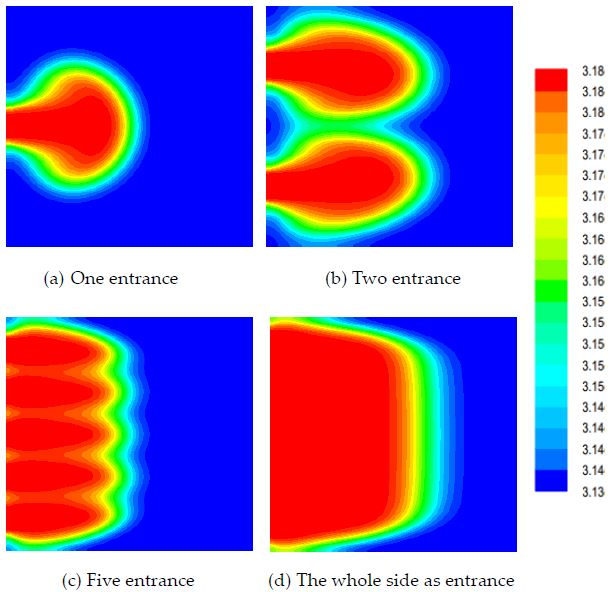
\includegraphics[width=12cm]{fig24.jpg}
\caption{The simulation results of different ways of arranging entrances} \label{fig24}
\end{figure}

From the above figure, the more the entrances are, the evener the temperature will be. Recalling on the before simulation outcome, when there is only one entrance for inflow, the temperature of corners is quietly lower than the middle area.

In conclusion, if we design more entrances, it will be easier to realize the goal to keep temperature even throughout the bathtub.

\item Model Application

Our before discussion is based on ideal assumptions. In reality, we have to make some corrections and improvement.

\begin{itemize}
\item[1)] Adding hot water continually with the mass flow of 0.16 kg/s. This way can ensure even mean temperature throughout the bathtub and waste less water.

\item[2)] The manufacturers can design an intelligent control system to monitor the temperature so that users can get more enjoyable bath experience.

\item[3)] We recommend users to add bubble additives to slow down the water being cooler and help cleanse. The additives with lower thermal conductivity are optimal.

\item[4)] The study method of our establishing model can be applied in other area relative to convection heat transfer, such as air conditioners.
\end{itemize}
\end{itemize}

\begin{thebibliography}{99}
\addcontentsline{toc}{section}{Reference}

\bibitem{1} Gi-Beum Kim. Change of the Warm Water Temperature for the Development of Smart Healthecare Bathing System. Hwahak konghak. 2006, 44(3): 270-276.
\bibitem{2} \url{https://en.wikipedia.org/wiki/Convective_heat_transfer#Newton.27s_law_of_cooling}
\bibitem{3} \url{https://en.wikipedia.org/wiki/Navier\%E2\%80\%93Stokes_equations}
\bibitem{4} \url{https://en.wikipedia.org/wiki/Computational_fluid_dynamics}
\bibitem{5} Holman J P. Heat Transfer (9th ed.), New York: McGraw-Hill, 2002. 
\bibitem{6} Liu Weiguo, Chen Zhaoping, ZhangYin. Matlab program design and application. Beijing: Higher education press, 2002. (In Chinese)

\end{thebibliography}

\newpage

\begin{letter}{Enjoy Your Bath Time!}

From simulation results of real-life situations, we find it takes a period of time for the inflow hot water to spread throughout the bathtub. During this process, the bath water continues transferring heat into air, bathtub and the person in bathtub. The difference between heat transfer capacity makes the temperature of various areas to be different. So that it is difficult to get an evenly maintained temperature throughout the bath water.

In order to enjoy a comfortable bath with even temperature of bath water and without wasting too much water, we propose the following suggestions.

\begin{itemize}
\item Adding hot water consistently
\item Using smaller bathtub if possible
\item Decreasing motions during bath
\item Using bubble bath additives
\item Arranging more faucets of inflow
\end{itemize}

\vspace{\parskip}

Sincerely yours,

Your friends

\end{letter}

\newpage

\begin{appendices}

\section{First appendix}

In addition, your report must include a letter to the Chief Financial Officer (CFO) of the Goodgrant Foundation, Mr. Alpha Chiang, that describes the optimal investment strategy, your modeling approach and major results, and a brief discussion of your proposed concept of a return-on-investment (ROI). This letter should be no more than two pages in length.

Here are simulation programmes we used in our model as follow.\\

\textbf{\textcolor[rgb]{0.98,0.00,0.00}{Input matlab source:}}
\lstinputlisting[language=Matlab]{./code/mcmthesis-matlab1.m}

\section{Second appendix}

some more text \textcolor[rgb]{0.98,0.00,0.00}{\textbf{Input C++ source:}}
\lstinputlisting[language=C++]{./code/mcmthesis-sudoku.cpp}

\end{appendices}
\end{document}
%%
%% This work consists of these files mcmthesis.dtx,
%%                                   figures/ and
%%                                   code/,
%% and the derived files             mcmthesis.cls,
%%                                   mcmthesis-demo.tex,
%%                                   README,
%%                                   LICENSE,
%%                                   mcmthesis.pdf and
%%                                   mcmthesis-demo.pdf.
%%
%% End of file `mcmthesis-demo.tex'.
